\newpage
\topic{3 continued}{Locate the velocity before interpolating it}
\begin{center}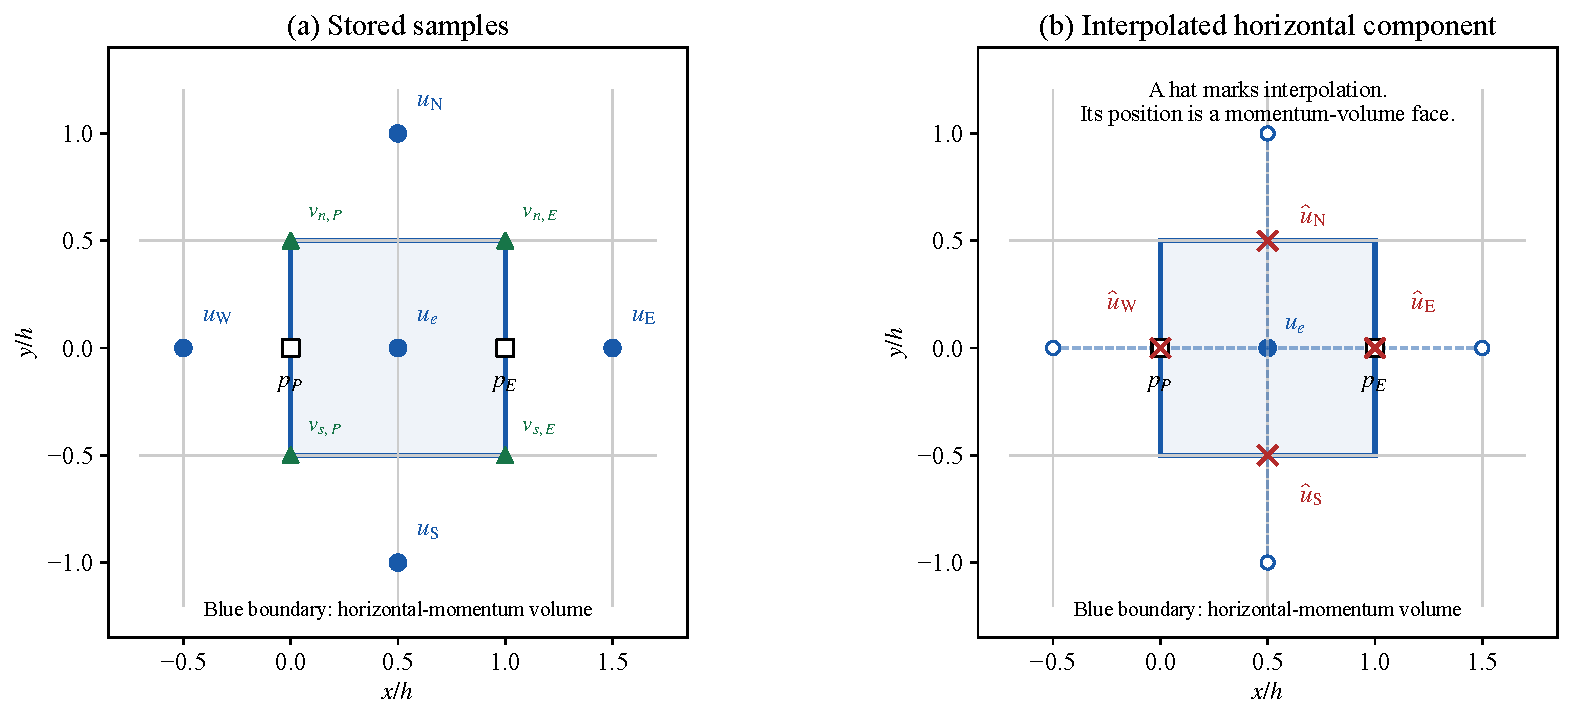
\includegraphics[width=\linewidth]{week01_2_assets/hat_locations.pdf}\end{center}
Use local coordinates with origin at pressure center $P$. The axes are measured in grid spacings $h$. The pressure
centers are $P=(0,0)$ and $E=(h,0)$. The horizontal velocity $u_e$ is stored
at $(h/2,0)$, on their shared pressure-cell face. Its own momentum control
volume is shifted: $0\leq x\leq h$ and $-h/2\leq y\leq h/2$.

The blue circles are stored horizontal components. The red crosses are
evaluation points at the faces of this momentum volume. In these face-flux formulas, a hat denotes
interpolation to a momentum-volume face. The east and west crosses coincide with pressure
centers; the north and south crosses lie at pressure-cell corners. These
geometrical coincidences do not make pressure and horizontal velocity the
same variable.

Each cross lies halfway between two blue samples. For example,
\[
\widehat u_{\rm N}=\frac{u_e+u_{\rm N}}2,\qquad
\widehat u_{\rm E}=\frac{u_e+u_{\rm E}}2.
\]
The subscript N on $u_{\rm N}$ means a neighboring \emph{horizontal} component
one grid spacing to the north. It does not mean a vertical velocity. The green
triangles store vertical components, which supply the speeds carrying fluid
through the north and south faces.

\textbf{Read each mark in its equation.} In the face-flux formulas a hat indicates interpolation; a star indicates
a provisional momentum solution; a prime indicates a pressure or velocity
correction. None of these marks independently identifies a pressure-cell center.
The later PIMPLE equations use $q_{\rm lag}^{(\ell)}$ and
$p_{\rm lag}^{(\ell)}$ for the latest outer-iteration estimates, keeping the hat
for spatial interpolation.
\newpage
\topic{3 continued}{Crossing a face while carrying horizontal momentum}
\begin{center}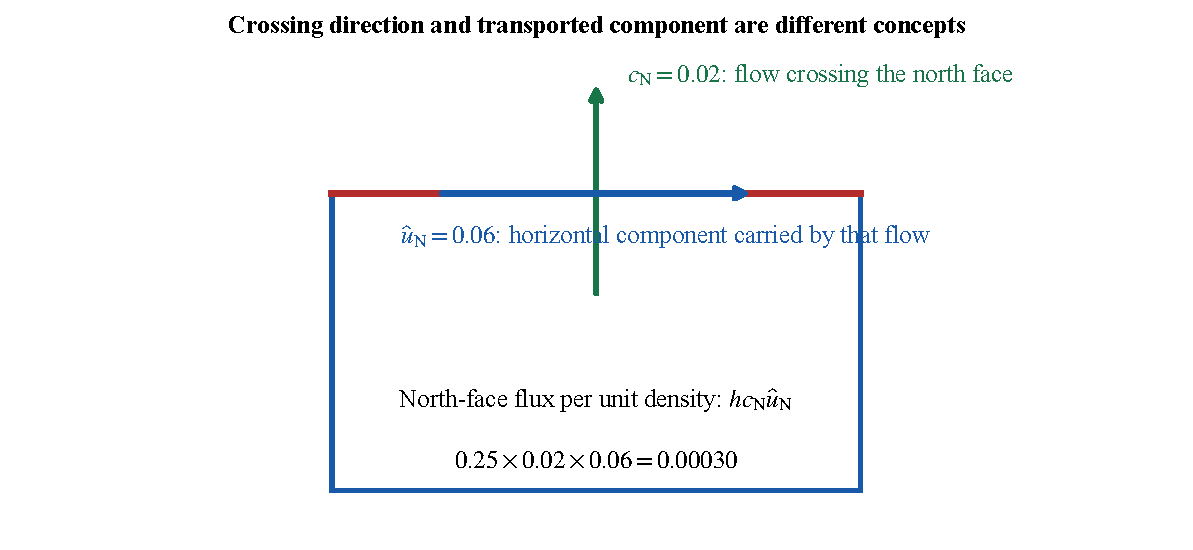
\includegraphics[width=\linewidth]{week01_2_assets/north_face_transport.pdf}\end{center}
At the north face, $c_{\rm N}$ is vertical: it carries fluid across the face.
The transported quantity $\widehat u_{\rm N}$ is horizontal. Per unit density
and unit depth, their product times the face length is the integrated
horizontal-momentum flux $h c_{\rm N}\widehat u_{\rm N}$.

\textbf{Arithmetic example.} Take nondimensional $h=0.25$ and the stored values
\[
(u_e,u_{\rm E},u_{\rm W},u_{\rm N},u_{\rm S})
=(0.04,0.12,0.02,0.08,-0.02).
\]
The four averages are
\[
(\widehat u_{\rm E},\widehat u_{\rm W},\widehat u_{\rm N},\widehat u_{\rm S})
=(0.08,0.03,0.06,0.01).
\]
Let the normal advecting speeds be $(c_{\rm E},c_{\rm W},c_{\rm N},c_{\rm S})
=(0.08,0.03,0.02,0.07)$. The north value averages $v_{n,P}=0.03$ and
$v_{n,E}=0.01$; the south value averages $v_{s,P}=0.05$ and $v_{s,E}=0.09$.
These values also satisfy continuity in the adjacent pressure cells $P$ and $E$.
The momentum volume's outward volume-flux balance is
$h(0.08-0.03+0.02-0.07)=0$. Its horizontal-momentum balance is different:
\begin{align*}
h(c_{\rm E}\widehat u_{\rm E}-c_{\rm W}\widehat u_{\rm W}
+c_{\rm N}\widehat u_{\rm N}-c_{\rm S}\widehat u_{\rm S})
&=0.001600-0.000225+0.000300-0.000175\\
&=0.001500.
\end{align*}
Dividing by area $h^2$ gives the convection term $0.024$. The notebook checks
these values. This is a local interpolation example, not a solved cavity field.

In a linear momentum predictor, advecting speeds $c$ are frozen coefficients;
the transported horizontal components are unknowns. At east and west their
averaging formulas have the same geometry, but their roles in the solve differ.
